\documentclass[11pt]{article}
\usepackage{amsmath, amssymb, amsthm, graphicx, geometry, listings, xcolor, url, enumitem, fancyhdr, multirow}
\geometry{margin=1in}
\definecolor{darkgreen}{rgb}{0,0.5,0}
\pagestyle{fancy}

\lhead{SFSU, CSC 645-01}
\chead{Spring 2025}
\rhead{Computer Networks}

\title{Homework 2}
\author{Bryan Lee\\922649673}
\date{April 8, 2025}

\begin{document}

\maketitle
\thispagestyle{fancy}

\section*{Questions}

% Answer variables
\newcommand{\answerOne}{\textbf{
    Three kinds of DNS servers and their functionalities in the hierarchy of DNS system (from textbook):
    \begin{enumerate}
        \item Root DNS Servers - These are the top-level DNS servers in the hierarchy responsible for directing DNS queries to the appropriate top-level domain (TLD) servers (e.g., .com, .edu).
        Although thousands of instances of root servers are distributed globally, they are all replicas of 13 root server identities, managed by 12 different organizations, 
        and coordinated through the Internet Assigned Numbers Authority.
        \item Top-level domain (TLD) servers - These servers are responsible for top-level domains such as .com, .edu, .org, etc., and all the country top-level domains such as uk, fr, ca, and jp. 
        They respond with the IP address of the authoritative DNS server for the requested domain name.
        \item Authoritative DNS Servers - These servers contains the actual DNS records for domain names under their authority. 
        It is an organization's own DNS server (e.g., sfsu.edu). 
        It provides authoritative hostname to IP mappings for organization's named host. 
        For example, dns.umass.edu is the authoritative server for gaia.cs.umass.edu, meaning it knows the IP address of gaia.cs.umass.edu.
    \end{enumerate}
    Now, if the host cs.sfsu.edu wants to know the IP address of gaia.cs.umass.edu, it will first query its local DNS server, dns.sfsu.edu, asking for the IP address. 
    Since, dns.sfsu.edu doesn't know the IP address of gaia.cs.umass.edu, it will query a root DNS server. 
    The root server replies with the IP address of the .edu TLD server. 
    Then, dns.sfsu.edu queries the .edu TLD DNS server, which replies with the IP address of the authoritative DNS server, dns.umass.edu. 
    Finally, dns.sfsu.edu queries dns.umass.edu, which knows and returns the IP address of gaia.cs.umass.edu. 
    The local DNS server then forwards this IP address back to the original host, cs.sfsu.edu. \\\\
    Order of operation:
    \begin{enumerate}
        \item cs.sfsu.edu $\rightarrow$ dns.sfsu.edu
        \item dns.sfsu.edu $\rightarrow$ root DNS server $\rightarrow$ TLD server (.edu) $\rightarrow$ dns.umass.edu
        \item dns.sfsu.edu $\leftarrow$ IP address of gaia.cs.umass.edu $\leftarrow$ dns.umass.edu
        \item cs.sfsu.edu $\leftarrow$ IP address from dns.sfsu.edu
    \end{enumerate}
}}

\newcommand{\answerTwo}{\textbf{
    We need to introduce sequence numbers to distinguish new packets from duplicate transmissions. 
    Sequence numbers help identify each packet uniquely, especially when packets are retransmitted, and preserve order in the case of out-of-order delivery. 
    This helps maintain the integrity of the data and avoid data corruption. 
    \\\\
    We need to introduce ACK/NAK to confirm the delivery of data packets. 
    ACK (acknowledgment) confirms the successful receipt of a packet. 
    On the contrary, NAK (negative acknowledgment) informs the sender that a packet was lost or contains an error. 
    These acknowledgments provide feedback to the sender to determine whether it needs to be retransmitted or the next packet should be continued sending. 
    \\\\
    We need to introduce timers to set a timeout period for detecting packet loss. 
    If an ACK is not received within the timeout, the sender retransmits the packer, assuming it was lost. 
    This ensures that the transmission does not hang for too long.
}}

\newcommand{\answerThreePartOne}{\textbf{
    The other packets will arrive to the sender but are discarded and no ACKs will be sent. 
    After the timeout, the sender will retransmit the first five packet.
    This happens as Go-Back-N requires the receiver only to accept the next expected in-order packet, so if a packet is lost, the subsequent packets are ignored, triggering a resend once timeout.
}}

\newcommand{\answerThreePartTwo}{\textbf{
    The sender doesn't receive any ACK, so after a timeout, it retransmits the first packet and all subsequent packets in the window, even if they were already received. 
    The receiver discards the duplicates and resends the missing ACK. 
    Once the sender receives the missing ACK, it sends the next window of packets.
}}

\newcommand{\answerThreePartThree}{\textbf{
    For Selective Repeat, when I dropped the first packet before it reached the destination, the receiver successfully received and buffered the other packets and sent out their respective ACKs. 
    However, no ACK was sent for the first packet. 
    After a timeout, the sender retransmitted the first packet, the receiver buffered it, and sent out its ACK. 
    Once the sender received the ACK, it moved on to the next batch.
    \\\\
    For the other case where I dropped the first ACK, it does the same thing as when I dropped the first packet.
    However, the only difference is that it sends out a DUPACK, which once recieved by the sender, will then transmit
    the next batch.
    \\\\
    Overall, Selective Repeat allows the receiver to accept out-of-order packets and buffer them compared to Go-Back-N.
}}

\newcommand{\answerFourPartOne}{\textbf{
    The first segment starts at the sequence number of 127 and contains 80 bytes. The second segment's sequence number is then: 127 + 80 = 207.
}}

\newcommand{\answerFourPartTwo}{\textbf{
    If the first segment of sequence number 127 and 80 bytes of data arrives first, Host B acknowledges the next expected byte: 127 + 80 = 207.
}}

\newcommand{\answerFourPartThree}{\textbf{
    If the second segment of sequence number 207 and 40 bytes of data arrives first, Host B still expects byte 127. 
    Since we are communicating via TCP, out-of-order segments do not update the ACK number, so the ACK number is 127.
}}

\newcommand{\answerFourPartFour}{\textbf{
    \begin{figure}[ht]
        \centering
        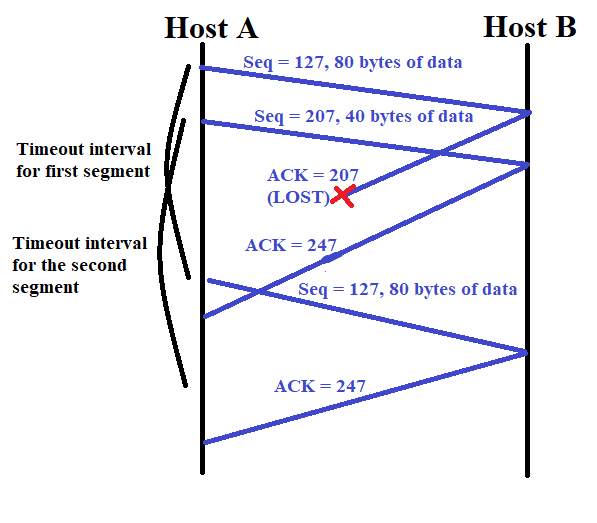
\includegraphics[width=0.9\linewidth]{TCP_Part_D.PNG}
        \caption{Part D Solution}
    \end{figure}
}}

\begin{enumerate}
    \item (20 Points) Describe the three kinds of DNS servers and their functionalities in the
    hierarchy of DNS system. Suppose the host cs.sfsu.edu wants to know the IP address of
    gaia.cs.umass.edu. Also suppose that the local DNS server of SFSU is called dns.sfsu.edu,
    and an authoritative DNS server for gaia.cs.umass.edu is called dns.umass.edu. Describe
    the interaction of the host and DNS servers (including the local DNS server). \\\\ \answerOne

    \item (15 Points) In the reliable data transfer protocols, why do we need to introduce sequence
    numbers? Why do we need to introduce ACK/NAK? Why do we need to introduce timers? \\\\ \answerTwo
    
    \item (40 Points) Visit the online animations for Go-Back-N and Selective Repeat.
        \begin{enumerate}[label=(\alph*)]
            \item Have the source send five packets, and then pause the animation before any of the five
            packets reach the destination. Then kill the first packet and resume the animation.
            Describe what happens and why. \\\\ \answerThreePartOne
            \item Repeat the experiment, but now let the first packet reach the destination and kill the
            first acknowledgment. Describe again what happens and why. \\\\ \answerThreePartTwo
            \item Repeat a and b with the Selective Repeat and answer the above questions again. \\\\ \answerThreePartThree
        \end{enumerate}
    
    \item (25 Points) Host A and B are communicating over a TCP connection, and Host B has
    already received all bytes up through byte 126 from A. Suppose Host A then sends two
    segments to Host B back-to-back. The first and second segments contain 80 and 40 bytes
    of data, respectively. In the first segment, the sequence number is 127. Host B sends an
    acknowledgment whenever it receives a segment from Host A.
        \begin{enumerate}[label=(\alph*)]
            \item In the second segment sent from Host A to Host B, what is the sequence number? \\\\ \answerFourPartOne
            \item If the first segment arrives before the second segment, in the acknowledgment of the first
            arriving segment, what is the acknowledgment number? \\\\ \answerFourPartTwo
            \item If the second segment arrives before the first segment, in the acknowledgment of the first
            arriving segment, what is the acknowledgment number? \\\\ \answerFourPartThree
            \item Suppose the two segments sent by A arrive in order at B. The first acknowledgment is lost
            and the second acknowledgment arrives after the first timeout interval. Draw a timing
            diagram, showing these segments and all other segments and acknowledgments sent.
            (Assume there is no additional packet loss.) For each segment in your figure, provide the
            sequence number; for each acknowledgment that you add, provide the acknowledgment
            number. \\\\ \answerFourPartFour
        \end{enumerate}
\end{enumerate}


\end{document}